% include the figures path relative to the master file
\graphicspath{ {./content/method/figures/} }

\section{Data}\label{sec:data}
\cite{giger2008anniversary}
\deleted[id=sik]{
  Despite Venhuizen et al. tested on a public dataset~\cite{dukeBIG}, this dataset is intended to AMD.
  Srinivasan also tested on a public dataset~\cite{dukeSmall}, however the images are cropped and filtered etc.
  So thats why we collected the SERI dataset.
}

The method is tested using a publicly available dataset of $384$ \gls{oct} volumes~\cite{VENHUIZEN_DATASET} ~\cite{Venhuizen2015}

Srinivasan\,\textit{et~al.}~\cite{Srinivasan2014} 
The images that have been used in their paper, are publicly available but are already preprocessed (i.e., denoised), have different sizes for the \gls{oct} volumes, do not offer a huge variability in term of \gls{dme} lesions, and some of them, without specifying which, have been excluded for the training phase; all these reasons prevent us from using this dataset to benchmark our work.


\added[id=old]{
This dataset was acquired by the Singapore Eye Research Institute (SERI), using
CIRRUS TM (Carl Zeiss Meditec, Inc., Dublin, CA) \gls{sdoct} device. The dataset
consists of 32 \gls{oct} volumes (16 \gls{dme} and 16 normal cases). Each volume
contains 128 B-scan with resolution of 512 $\times$ 1024 pixels.  All
\gls{sdoct} images are read and assessed by trained graders and identified as
normal or \gls{dme} cases based on evaluation of retinal thickening, hard
exudates, intraretinal cystoid space formation and subretinal fluid.
}

\begin{figure}
  \centering{
    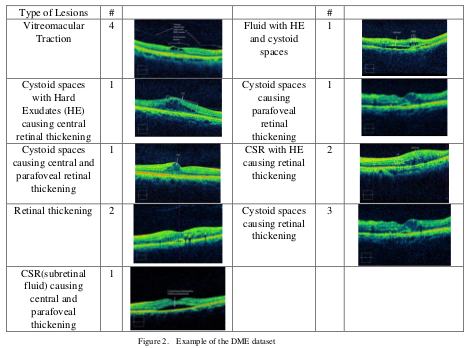
\includegraphics[width=1\linewidth]{bbdd}}
    \caption{Experimental Setup}
  \label{fig:ML-scheme}
\end{figure}
